\chapter{Grundlagen}

\section{Generative Adversarial Networks}
Generative Adversarial Networks, kurz GANs, sind eine aufstrebende Technologie im Bereich des maschinellen Lernens und der künstlichen Intelligenz. Inspiriert von Ian Goodfellow und seinen Kollegen im Jahr 2014, bieten GANs eine effiziente Möglichkeit, tiefe Repräsentationen von Daten zu erlernen, ohne dass große Mengen an annotierten Trainingsdaten benötigt werden\cite{Creswell.2018}. 
Dies wird durch die Verwendung von Backpropagation und den Wettbewerb zwischen zwei neuronalen Netzen - dem Generator und dem Diskriminator - erreicht. 
Daraus ergeben sich zahlreiche neue Ansätze zur Generierung realistischer Inhalte. 
Die Anwendungen reichen von der Bildgenerierung bis hin zur Superauflösung und Textgenerierung \cite{Aggarwal.2021}.

\subsection{Funktionsweise}
Der Generator und der Diskriminator sind die Hauptkomponenten eines GAN. Die beiden neuronalen Netze werden gleichzeitig trainiert und konkurrieren miteinander, wobei der Generator versucht, den Diskriminator zu täuschen, indem er synthetische Inhalte erzeugt. Um die Glaubwürdigkeit des Generators zu erhöhen, so dass der Diskriminator nicht mehr zwischen den Eingaben unterscheiden kann, wird das gesamte Netz trainiert. Die Netze werden in der Regel als mehrschichtige Netzwerke implementiert, die aus Convolutional und Fully-Connected Schichten bestehen\cite{Creswell.2018}.

\subsubsection*{Generator}
Der Generator dient zur Erzeugung künstlicher Daten wie Bilder und Texte. 
Der Generator ist nicht mit dem realen Datensatz verbunden und lernt daher nur durch die Interaktion mit dem Diskriminator. Wenn der Diskriminator nur noch 50\% der Eingaben richtig vorhersagt, gilt der Generator als optimal\cite{Creswell.2018}.

\subsubsection*{Diskriminator}
Die Unterscheidung zwischen echten und unechten Eingaben ist Aufgabe des Diskriminators. Der Diskriminator kann sowohl künstliche als auch reale Daten verwenden. 
Wenn der Diskriminator nicht mehr richtig unterscheiden kann, wird er als konvergierend bezeichnet\cite{Aggarwal.2021}. Andernfalls wird er als optimal bezeichnet, wenn seine Klassifizierungsgenauigkeit maximiert ist. Im Falle eines optimalen Diskriminators wird das Training des Diskriminators gestoppt und der Generator trainiert alleine weiter, um die Genauigkeit des Diskriminators wieder zu verbessern\cite{Creswell.2018}.

\subsection{Training}
Das Training besteht in der Optimierung der Parameter für sowohl den Generator als auch den Diskriminator durch die Anwendung von Backpropagation zur Verbesserung dieser Parameter. Dieses Verfahren wird häufig als anspruchsvoll und instabil beschrieben. Einerseits gestaltet sich die Herausforderung, beide Modelle konvergieren zu lassen. Andererseits besteht die Problematik darin, dass der Generator Muster erzeugen kann, die für verschiedene Eingaben äußerst ähnlich sind, was als "Mode-Collapse-Problem" bekannt ist. Der Diskriminatorverlust kann sich rasch gegen Null konvergieren, wodurch ein zuverlässiger Gradientenfluss für die Aktualisierung des Generators verhindert wird.
Zur Bewältigung dieser Herausforderungen wurden verschiedene Lösungsansätze vorgeschlagen. Ein Beispiel ist die Verwendung heuristischer Verlustfunktionen. Eine alternative Strategie, die von Sonderby et al. vorgeschlagen wurde, besteht darin, den Datensatz vor der Verwendung zu verrauschen \cite{Creswell.2018}.

\subsubsection*{Adversarieller Verlust}
Der adversarielle Verlust, auch als GAN-Verlust bekannt, spielt eine zentrale Rolle im Trainingsprozess. Dieser Verlust basiert auf dem Konzept des Minimax-Spiels zwischen dem Generator und dem Diskriminator. Der Generator strebt danach, den Diskriminator zu überlisten und Daten zu erzeugen, die von echten Daten nicht zu unterscheiden sind. Gleichzeitig ist es das Ziel des Diskriminators, zwischen echten und generierten Daten zu differenzieren. Der adversarielle Verlust wird in der Gleichung 2.1 repräsentiert.

\begin{equation}
    \min_G \max_D V(D, G) = \mathbb{E}_{x\sim p_{\text{data}}(x)}[\log D(x)] + \mathbb{E}_{z\sim p_z(z)}[\log(1 - D(G(z)))]
\end{equation}

Hierbei bezeichnet $G$ den Generator, $D$ den Diskriminator, $x$ echte Daten, $z$ das Rauschen und $p_{data}$ sowie $p_z$ die Wahrscheinlichkeitsverteilungen von echten Daten und Rauschen. Der Minimax-Ansatz impliziert, dass der Generator versucht, den Verlust zu minimieren, während der Diskriminator versucht, ihn zu maximieren. Eine gezielte Optimierung und Anpassung des adversariellen Verlusts ist entscheidend, um Herausforderungen wie dem Mode-Collapse-Problem und den Konvergenzproblemen zu begegnen \cite{Hong.2020}.

\subsection{Anwendungen}
GANs wurden ursprünglich im Kontext des unüberwachten maschinellen Lernens konzipiert, haben jedoch herausragende Leistungen sowohl im halbüberwachten Lernen als auch im Reinforcement Learning gezeigt \cite{Aggarwal.2021}. Diese Vielseitigkeit hat dazu geführt, dass GANs in verschiedenen Domänen wie dem Gesundheitswesen und dem Bankwesen Anwendung finden.

Im Bereich der medizinischen Bildgebung bieten GANs innovative Lösungsansätze, um den Herausforderungen von Datenknappheit und Patientenprivatsphäre zu begegnen. Von der Erkennung und Behandlung chronischer Krankheiten über die Segmentierung bis hin zur Bildrekonstruktion können GANs vielfältige Anwendungen haben. Zahlreiche GAN-Ansätze wurden bereits entwickelt, um die Rauschunterdrückung in medizinischen Bildverfahren zu verbessern, was wiederum die Qualität von Diagnosen steigern kann \cite{Yi.2019}. Darüber hinaus werden GANs nicht nur im Gesundheitswesen, sondern auch in anderen Bereichen eingesetzt, insbesondere in der Bildsynthese. 

In der Finanzindustrie helfen GANs, das Handels- und Risikomanagement zu verbessern, indem sie synthetische Zeitreihen erzeugen, die wichtige Finanzdaten widerspiegeln \cite{Eckerli.2021}. Zheng et al. (2018) schlugen beispielsweise eine GAN vor, die auf dem Telekommunikations-Betrugsfall in China im Jahr 2017 basiert und die Wahrscheinlichkeit berechnet, wann eine Überweisung betrügerisch sein könnte \cite{Zheng.2018}. 

Des Weiteren wurden Forschungsanstrengungen unternommen, um mittels GANs menschliche Bewegungen vorherzusagen, insbesondere anhand von 3D-Skelett-\\sequenzen \cite{Jain.2020}. Zudem ermöglichen GANs die Identifikation von 3D-Objekten sowie die Generierung realistischer Bilder und Texte in verschiedenen Anwendungsbereichen \cite{Aggarwal.2021}.
Die Vielseitigkeit von GANs eröffnet somit ein breites Spektrum an Potenzialen für verschiedene Anwendungsbereiche.

\subsection{Limitationen}
Ein kritisches Problem von GANs ist die Instabilität des Trainings aufgrund von Mode-Collapse, was die Weiterentwicklung des generativen Lernens und potentielle Anwendungen einschränkt\cite{Liu.2022}. Der Generator lernt nur Bilder bestimmter Arten der Datenverteilung.  Andere Arten, die ebenfalls in der Verteilung vorkommen, werden hingegen vernachlässigt\cite{Srivastava.2017}. Ansätze wie das Hinzufügen von Rauschen zum Netzwerk, eine Manifold Entropy Estimation \cite{Liu.2022} und implizites Variationslernen \cite{Srivastava.2017} wurden bereits vorgeschlagen, um dieses Problem zu lösen.
Des Weiteren birgt die Fähigkeit eines GANs zur Generierung von Inhalten, die nahezu identisch mit authentischen Inhalten sind, potenzielle Herausforderungen in realen Szenarien, insbesondere im Zusammenhang mit der menschlichen Bildsynthese. Diese Fähigkeit ermöglicht es Betrügern, gefälschte Profile in sozialen Medien zu erstellen. Gezielte Anwendungen von GANs, die darauf ausgelegt sind, einzigartige und realistische Bilder von Personen zu erzeugen, die in der Realität nicht existieren, könnten die Erstellung falscher Profile erschweren\cite{Aggarwal.2021}.


\section{Pix2Pix}
Pix2Pix hat sich als zentrales Framework für Bild-zu-Bild-Übersetzungen auf der Basis von bedingten generativen adversariellen Netzwerken (cGANs) etabliert. Es ermöglicht die Erstellung einer abstrakten Abbildung von einem Eingangsbild zu einem korrespondierenden Ausgangsbild und bewältigt dabei eine vielfältige Palette an Bildübersetzungsaufgaben, wie die Transformation von Skizzen in realistische Bilder oder die Konvertierung von Tages- zu Nachtaufnahmen.
  

\subsection{Pix2Pix-Kernkonzepte}
Die Bildverarbeitung hat in den letzten Jahren durch den Einsatz tiefer neuronaler Netzwerke erhebliche Fortschritte gemacht. Im Mittelpunkt vieler dieser Fortschritte steht die U-Net-Architektur, die speziell für die Bildsegmentierung entwickelt wurde. Diese Architektur zeichnet sich durch ihre angeklügelte Kombination aus Encoder- und Decoder- Strukturen sowie durch den Einsatz von Skip-Verbindungen aus.
 \newline
Bei der Encoder-Decoder-Struktur handelt es sich um einen Ansatz, bei dem das Eingangsbild zunächst durch den Encoder schrittweise reduziert wird. Dieser Prozess dient dazu, wesentliche Merkmale des Bildes zu erfassen. Anschließend wird das Bild durch den Decoder wiederhergestellt, indem die zuvor extrahierten Merkmale verwendet werden. Während dieser Prozesse besteht jedoch das Risiko des Informationsverlustes, insbesondere in den tieferen Schichten des Netzwerks.
Um dieses Problem zu adressieren, führt die U-Net-Architektur Skip-Verbindungen ein. Diese direkten Verbindungen zwischen korrespondierenden Schichten des Encoders und Decoders sorgen dafür, dass Detailinformationen nicht verloren gehen. Genauer gesagt, ermöglichen diese Verbindungen den direkten Informationsfluss zwischen jeweils äquivalenten Schichten, wodurch die Rekonstruktion des Bildes im Decoder mit einer höheren Genauigkeit erfolgt. \newline
Die Bedeutung von Skip-Verbindungen zeigt sich insbesondere in Anwendungen wie der Bild-zu-Bild-Übersetzung. Hier muss oft ein Bild mit niedriger Auflösung in ein Bild mit hoher Auflösung überführt werden, ohne dass Details verloren gehen. Die U-Net-Architektur, die angereichert mit diesen Verbindungen ist, ermöglicht daher eine feinere Rekonstruktion, die sowohl globale als auch lokale Informationen berücksichtigt. \newline
Somit kann die U-Net-Architektur durch ihre Kombination aus Encoder-Decoder-Struktur und Skip-Verbindungen ein effektives Werkzeug für die Bildsegemtierung darstellen. Ihre Fähigkeit, sowohl globale Muster als auch feine Details zu berücksichtigen, macht sie zu einer bevorzugten Wahl für viele Bildverarbeitungsaufgaben. \newline
In Abbildung \ref{fig:unet} ist die typische U-Net-Architektur dargestellt. Die linke Seite des ''U'' repräsentiert den Encoder-Teil, der das Eingangsbild schrittweise reduziert und wesentliche Merkmale extrahiert. Die rechte Seite repräsentiert den Decoder-Teil, der das Bild mithilfe der extrahierten Merkmale rekonstruiert. Die horizontalen Linien repräsentieren die Skip-Verbindungen, die sicherstellen, dass Detailinformationen zwischen den korrespondierenden Schichten des Encoder und Decoders direkt übertragen werden. \newline 
In der Pix2Pix Technologie dient diese U-Net-Architektur als Generator. Er ist das zentrale Element, das für die Bild-zu-Bild-Übersetzung verantwortlich ist. Die Wahl der U-Net-Struktur für den Generator liegt in ihrer Fähigkeit, feinere Details und Kontextinformationen aus dem Eingangsbild beizubehalten, was für die Bild-zu-Bild-Übersetzung von entscheidender Bedeutung ist. Die Encoder-Decoder-Struktur des U-Net ermöglicht es dem Generator, den globalen Kontext des Bildes zu erfassen, während die Skip-Verbindungen sicherstelle, dass auch lokale Details im resultierenden Bild berücksichtigt werden.

\begin{figure}[h]
	\centering
	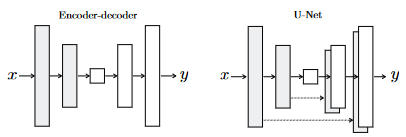
\includegraphics[width=0.7\linewidth]{./images/unet.png}
	\caption{Schematische Darstellung der U-Net-Architektur. Die Architektur besteht aus einem Encoder-Teil (links), einem Decoder-Teil (rechts) und Skip-Verbindungen zwischen korrespondierenden Schichten.}
	\label{fig:unet}
\end{figure}

\subsection{Anwendungen von Pix2Pix}
Pix2Pix ist eine fortschrittliche Methode für Bild-zu-Bild-Übersetzungsaufgaben und hat eine breite Palette von Anwendungen in der Bildverarbeitung.\newline
Ein markantes Anwendungsbeispiel ist die Umwandlung von architektonische Entwürfe oder Zeichnungen in realistische Gebäudefotos. Besonders eindrucksvoll ist diese Anwendung beim CMP Facades-Datensatz, wo aus simplen Fassadenzeichnungen detailreiche Gebäudebilder generiert werden. \cite{PhillipIsola.}
\newline
Im Bereich der Fotografie wird Pix2Pix verwendet, um Schwarz-Weiß-Fotos in farbige Bilder zu konvertieren, was besonders bei der Restaurierung alter Fotografien von Bedeutung sein kann.
\newline
Die Transformation von Tagesaufnahmen in Nachtbilder ist eine weitere beeindruckende Leistung von Pix2Pix sowie die Umwandlung von Thermalaufnahmen in Farbfotos.
\newline
Schließlich wird Pix2Pix auch zur Vervollständigung von Fotos mit fehlenden Pixeln verwendet, beispielsweise um unvollständige Bilder, die aus Paris StreetView stammen, zu reparieren und zu vervollständigen.
\newline
Diese vielfältigen Anwendungen zeigen die enorme Flexibilität und die breite Einsatzmöglichkeit von Pix2Pix in der modernen Bildbearbeitung und Computergrafik.
 

\section{CycleGAN}
CycleGAN, das 2017 von Jun-Yan Zhu et al. vorgestellt wurde, stellt eine neue Entwicklung im Bereich des maschinellen Lernens und insbesondere der Bildübersetzung zwischen unpaaren Domänen dar. Es erweitert die Pix2Pix-Architektur durch die Einführung einer Zykluskonsistenz-Verlustfunktion (Cycle Consistency Loss), die sicherstellt, dass das Originalbild nach einem Übersetzungs- und Rückübersetzungszyklus erhalten bleibt. Der Generator $G$ transformiert Bilder aus der Domäne $X$ in die Domäne $Y$, während der Generator $F$ den umgekehrten Prozess durchführt. Diese Transformationen werden ohne gepaarte Trainingsdaten durchgeführt.

\subsection{CycleGAN - Kernkonzepte}
\chapter*{Cycle GAN}

CycleGAN ist ein leistungsstarkes Modell im Bereich des maschinellen Lernens, das darauf abzielt, Bildübersetzungen zwischen verschiedenen Domänen ohne die Notwendigkeit für gepaarte Daten durchzuführen. Diese Technik wurde erstmals 2017 von Jun-Yan Zhu et al. in ihrer bahnbrechenden Arbeit "Unpaired Image-to-Image Translation using Cycle-Consistent Adversarial Networks" vorgestellt. Dieses Kapitel widmet sich der Funktionsweise von CycleGAN und seinen vielfältigen Anwendungen.

\subsection*{Funktionsweise von CycleGAN}

CycleGAN basiert auf dem GAN-Prinzip. Der Generator erzeut Bilder, während der Diskriminator zwischen den echten und generierten Bilder unterscheiden muss. Im Falle von CycleGAn wird das Modell erweitert, um die Übersetzung zwischen zwei Domänen $X$ und $Y$ zu ermöglichen. 

\subsection*{Generator}

\subsection*{Diskriminator}

\subsection*{Cycle - Konsistenz}

\subsection*{Verlustfunktionen}


\section{Convolutional Layers}
Convolutional Layers repräsentieren eine fundamentale Komponente innerhalb neuronaler Netzwerke, insbesondere im Kontext der Verarbeitung von Bildinformationen. Diese Schicht nutzt Convolution-Operationen, um durch Faltung von Eingabedaten mit Filterkernen lokale Muster zu identifizieren. Die Filterkerne, üblicherweise in Größen wie 3x3, 7x7 oder 9x9, fungieren als kleine Arrays und dienen der Extraktion spezifischer Merkmale im Bild.

Die Funktionsweise dieser Schicht basiert auf der schrittweisen Verschiebung der Filterkerne über das Eingangsbild. An den jeweiligen Pixelpositionen erfolgt eine präzise elementweise Multiplikation, gefolgt von einer anschließenden Summation aller resultierenden Werte. Diese berechneten Werte werden dann in den korrespondierenden Positionen der Feature Map eingetragen, wie in der Abbildung \ref{fig:convolutionalLayer} veranschaulicht. Durch diesen Prozess gewinnen tiefere Schichten des Netzwerks die Fähigkeit, zunehmend komplexe und abstrakte Informationen auf höheren Ebenen der Hierarchie zu repräsentieren.

\begin{figure}[ht]
	\centering
	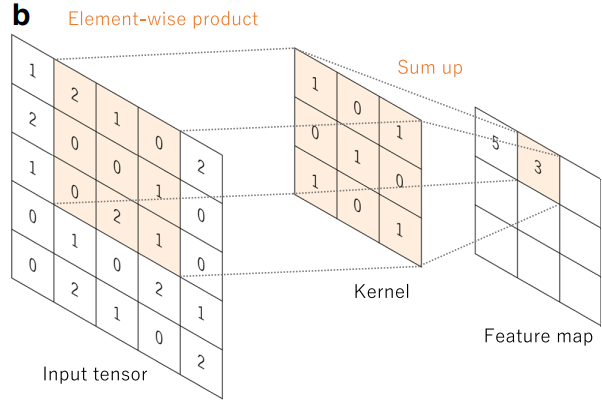
\includegraphics[width=0.5\linewidth]{./images/convolutionalLayer.png}
	\caption{Beispiel einer Convolutional-Operation mit einem 3x3 Kernel und Stride 1}
	\label{fig:convolutionalLayer}
\end{figure}

Die Verwendung verschiedener Kernels, sowohl in Bezug auf Größe als auch Anzahl, erlaubt die Extraktion vielfältiger Merkmale wie Kanten oder Texturen. Diese Flexibilität befähigt das Netzwerk, auf unterschiedlichste visuelle Strukturen ansprechend zu reagieren \cite{Yamashita.2018}.

Zusätzlich fungieren die Kernels als Subsampling-Mechanismus, bedingt durch die begrenzte Ausdehnung der Convolution-Operation bis zum Bildrand. Die Wahl der Strides, als die Distanz zwischen zwei verschobenen Kernelpositionen, beeinflusst diesen Subsampling-Effekt. Die Anwendung von Padding, um das Bild vor jeder Convolution zu vergrößern, kann dazu beitragen, ungewollte Unterabtastung (Downsampling) zu minimieren.

Ein wesentlicher Vorzug von Convolutional Layers besteht in der signifikanten Reduzierung der zu trainierenden Parameter und der Komplexität des Modells. Dies führt zu einer verbesserten Effizienz, da weniger Gewichte optimiert werden müssen, und trägt zur Prävention von Overfitting bei\cite{Yamashita.2018,OShea.2015}.

Die Ergebnisse der Convolutional Layer werden anschließend durch eine nicht-lineare Aktivierungsfunktion weitergereicht, um die Fähigkeit des Netzwerks zur Modellierung komplexer, nicht-linearer Zusammenhänge zu verbessern. Die Einbeziehung einer Aktivierungsfunktion, wie beispielsweise der ReLU (Rectified Linear Unit), ermöglicht es dem Netzwerk, nicht-linear separierbare Muster und Merkmale zu erfassen. Ohne Aktivierungsfunktionen würden die Convolutional Layers nur lineare Transformationen durchführen, was die Lernfähigkeit des Modells deutlich einschränken würde\cite{Sharma.2017}.

\section{Bibliotheken}
\subsection{Tensorflow}
TensorFlow ist ein weit verbreitetes Open-Source-Framework, das für maschinelles Lernen und tiefe neuronale Netzwerke eingesetzt wird\footnote{https://www.tensorflow.org/}. Es bietet eine umfangreiche Plattform zur Entwicklung und Umsetzung von Modellen in verschiedenen Anwendungsbereichen, darunter Bilderkennung und natürliche Sprachverarbeitung. Die Architektur von TensorFlow ermöglicht das Erstellen komplexer maschineller Lernanwendungen und stellt umfassende Tools und Bibliotheken zur Verfügung, um den gesamten Entwicklungsprozess zu unterstützen. Darüber hinaus profitiert TensorFlow von einer aktiven und engagierten Community, die kontinuierlich zur Weiterentwicklung des Frameworks beiträgt\footnote{https://github.com/tensorflow/tensorflow}.

\subsection{Keras}
Ursprünglich als eigenständiges Framework konzipiert und seit TensorFlow 2.0 in die TensorFlow Core API integriert, fungiert Keras als Open-Source-API zur Modellierung von Strukturen im Bereich des Deep Learning\footnote{https://www.tensorflow.org/guide/keras}. Diese Bibliothek, die in der Programmiersprache Python implementiert ist, umfasst sämtliche Phasen des maschinellen Lern-Workflows. Beginnend mit der Datenverarbeitung ermöglicht sie eine Fortführung bis zur präzisen Abstimmung der Hyperparameter während des Trainingsprozesses. Die Keras-Prinzipien zeichnen sich durch Einfachheit, Flexibilität und Leistungsfähigkeit aus und ermöglichen es den Anwendern, die Skalierbarkeit und plattformübergreifenden Fähigkeiten der TensorFlow-Plattform zu nutzen.\footnote{https://keras.io/about/}.